\documentclass[12pt,a4paper]{article}

% ─── Page Layout ───────────────────────────────────────────────────────────────
\usepackage[a4paper, margin=0.8in, headheight=14pt]{geometry}

% ─── Fonts (XeLaTeX) ───────────────────────────────────────────────────────────
\usepackage{fontspec}
\usepackage{unicode-math}
\setmainfont{TeX Gyre Pagella}
\setmonofont[Scale=0.88]{TeX Gyre Cursor}
\setmathfont{Latin Modern Math}

% ─── Packages ──────────────────────────────────────────────────────────────────
\usepackage{xcolor}
\usepackage{colortbl}
\usepackage{titlesec}
\usepackage{enumitem}
\usepackage{tabularx}
\usepackage{booktabs}
\usepackage{array}
\usepackage{amsmath}
\usepackage{tikz}
\usetikzlibrary{shapes.geometric, arrows.meta, positioning, calc, fit, decorations.pathreplacing}
\usepackage{tcolorbox}
\tcbuselibrary{skins, breakable}
\usepackage{hyperref}
\usepackage{fancyhdr}
\usepackage{graphicx}
\usepackage{microtype}
\hyphenpenalty=10000
\exhyphenpenalty=10000
\sloppy
\usepackage{caption}
\usepackage{setspace}
\usepackage{multirow}
\usepackage{tocloft}

% ─── Q&A helper ────────────────────────────────────────────────────────────────
\newcommand{\Q}[1]{\textbf{#1}\par\noindent\ignorespaces}

% ─── Colour Palette ────────────────────────────────────────────────────────────
\definecolor{myred}{RGB}{196,30,58}
\definecolor{mydark}{RGB}{30,30,50}
\definecolor{mygreen}{RGB}{14,120,80}
\definecolor{myteal}{RGB}{0,130,140}
\definecolor{myamber}{RGB}{180,100,0}
\definecolor{mypurple}{RGB}{100,30,160}
\definecolor{mygray}{RGB}{246,247,249}
\definecolor{mgframe}{RGB}{180,185,200}
\definecolor{watermark}{RGB}{145,150,170}
\definecolor{hdrred}{RGB}{250,232,235}
\definecolor{hdrgreen}{RGB}{220,244,233}
\definecolor{hdrteal}{RGB}{220,242,244}
\definecolor{hdramber}{RGB}{253,242,215}
\definecolor{hdrpurple}{RGB}{238,228,255}
\definecolor{hdrgray}{RGB}{238,240,245}
\definecolor{rowalt}{RGB}{250,251,253}

% ─── Section Formatting ────────────────────────────────────────────────────────
\titleformat{\section}
  {\large\bfseries\color{myred}}{\thesection.}{0.5em}{}
  [\vspace{1pt}{\color{myred}\rule{\linewidth}{0.8pt}}]
\titleformat{\subsection}
  {\normalsize\bfseries\color{myteal}}{\thesubsection}{0.5em}{}
\titlespacing*{\section}{0pt}{18pt}{7pt}
\titlespacing*{\subsection}{0pt}{11pt}{4pt}

% ─── Paragraph ─────────────────────────────────────────────────────────────────
\setlength{\parindent}{0pt}
\setlength{\parskip}{4pt}

% ─── TOC Styling ───────────────────────────────────────────────────────────────
\renewcommand{\cfttoctitlefont}{\large\bfseries\color{myred}}
\renewcommand{\cftaftertoctitle}{\par\noindent{\color{myred}\rule{\linewidth}{0.8pt}}}
\setlength{\cftbeforetoctitleskip}{0pt}
\setlength{\cftaftertoctitleskip}{6pt}
\renewcommand{\cftsecfont}{\normalsize\bfseries\color{mydark}}
\renewcommand{\cftsecpagefont}{\normalsize\bfseries\color{mydark}}
\renewcommand{\cftsecleader}{\cftdotfill{\cftdotsep}}
\setlength{\cftbeforesecskip}{7pt}
\renewcommand{\cftsubsecfont}{\small\color{mydark}}
\renewcommand{\cftsubsecpagefont}{\small\color{mydark}}
\setlength{\cftbeforesubsecskip}{3pt}
\setlength{\cftsubsecindent}{1.4em}

% ─── Table helpers ─────────────────────────────────────────────────────────────
\renewcommand{\arraystretch}{1.45}
\setlength{\tabcolsep}{6pt}
\arrayrulecolor{mydark}
\newcolumntype{B}[1]{>{\small\bfseries\raggedright\arraybackslash}m{#1}}
\newcolumntype{Y}{>{\small\raggedright\arraybackslash}X}
\renewcommand{\tabularxcolumn}[1]{m{#1}}

% ─── Header / Footer ───────────────────────────────────────────────────────────
\pagestyle{fancy}
\fancyhf{}
\fancyhead[L]{\small\color{myred}\textbf{PE-EC702B}\;\color{mydark}--- Digital Image and Video Processing}
\fancyhead[R]{\small\color{myteal}\textbf{Module 6 Notes}}
\fancyfoot[C]{\small\color{mydark}\thepage}
\fancyfoot[R]{\small\color{watermark}\textit{\copyright\ Biraj}}
\renewcommand{\headrulewidth}{0.5pt}
\renewcommand{\footrulewidth}{0.3pt}

% ─── Hyperref ──────────────────────────────────────────────────────────────────
\hypersetup{
  colorlinks=true, linkcolor=myteal, urlcolor=myteal,
  pdfauthor={Biraj Sarkar},
  pdftitle={PE-EC702B --- Module 6 Notes}
}

% ─── tcolorbox styles ──────────────────────────────────────────────────────────
\tcbset{
  tikzbox/.style={
    colback=mygray, colframe=mgframe, boxrule=0.6pt, arc=4pt,
    left=8pt, right=8pt, top=6pt, bottom=6pt,
    colbacktitle=mgframe, coltitle=mydark,
    fonttitle=\small\bfseries
  },
  defbox/.style={
    colback=hdrgreen, colframe=mygreen, boxrule=0.8pt, arc=4pt,
    left=9pt, right=9pt, top=6pt, bottom=6pt,
    colbacktitle=mygreen, coltitle=white,
    fonttitle=\small\bfseries
  },
  formulabox/.style={
    colback=hdrteal, colframe=myteal, boxrule=0.8pt, arc=4pt,
    left=9pt, right=9pt, top=7pt, bottom=7pt,
    colbacktitle=myteal, coltitle=white,
    fonttitle=\small\bfseries
  },
  examplebox/.style={
    colback=hdramber, colframe=myamber, boxrule=0.8pt, arc=4pt,
    left=9pt, right=9pt, top=6pt, bottom=6pt,
    colbacktitle=myamber, coltitle=white,
    fonttitle=\small\bfseries,
    breakable
  },
  masonbox/.style={
    colback=hdrpurple, colframe=mypurple, boxrule=0.8pt, arc=4pt,
    left=9pt, right=9pt, top=6pt, bottom=6pt,
    colbacktitle=mypurple, coltitle=white,
    fonttitle=\small\bfseries
  },
  exambox/.style={
    colback=hdrpurple, colframe=mypurple, boxrule=1pt, arc=5pt,
    left=10pt, right=10pt, top=8pt, bottom=8pt,
    colbacktitle=mypurple, coltitle=white,
    fonttitle=\bfseries,
    breakable, title after break={\textbf{Frequently Asked / Viva Questions (contd.)}}}
}
\tcbset{breakable}

% ─── TikZ styles ───────────────────────────────────────────────────────────────
\tikzset{
  block/.style={rectangle, draw=myteal, fill=hdrteal,
    text width=2.1cm, align=center, minimum height=0.85cm,
    font=\small, rounded corners=3pt, line width=0.7pt},
  arrow/.style={-Stealth, thick, color=mydark},
  line/.style={thick, color=mydark}
}

% ═══════════════════════════════════════════════════════════════════════════════
\begin{document}
% ═══════════════════════════════════════════════════════════════════════════════

\begin{center}
  {\LARGE\bfseries\color{myred} PE-EC702B --- Digital Image and Video Processing}\\[5pt]
  {\normalsize\color{mydark} Semester VII \quad$\bullet$\quad 3L:0T:0P \quad$\bullet$\quad 3 Credits}\\[3pt]
  {\normalsize\color{myteal}\textbf{Module 6 Exam Notes: Image Compression}}\\[3pt]
  {\small\color{mydark} CGEC \;$|$\; B.Tech ECE (2023--27) \;$|$\; \textit{Biraj Sarkar}}
\end{center}
\vspace{2pt}
\noindent{\color{myred}\rule{\linewidth}{1.5pt}}
\vspace{2pt}

\hypersetup{linkcolor=mydark}
\tableofcontents
\hypersetup{linkcolor=myteal}
\newpage

% ===============================================================================
\section{Redundancies in Digital Images}
% ===============================================================================

Data compression reduces the amount of data required to represent a given quantity of information by identifying and eliminating statistical redundancies.

\begin{tcolorbox}[defbox, title={Types of Image Redundancy}]
\begin{itemize}[leftmargin=*, itemsep=3.5pt]
  \item \textbf{Coding Redundancy:} Occurs when the codes assigned to gray levels do not minimize average code word length. Resolved by assigning shorter codes to highly probable intensities (entropy coding).
  \item \textbf{Inter-pixel (Spatial) Redundancy:} Results from the high correlation between adjacent pixels. We compress by encoding differences rather than absolute values (predictive coding).
  \item \textbf{Psycho-visual Redundancy:} Information that is ignored by the human visual system (e.g., fine details in highly textured or colored areas). Quantization represents this lossy elimination.
\end{itemize}
\end{tcolorbox}

% ===============================================================================
\section{Lossless Compression Methods}
% ===============================================================================

Lossless compression allows perfect reconstruction of the original image.

\subsection{Lossless Predictive Coding}
Based on eliminating inter-pixel redundancy. We predict the current pixel value $\hat{f}(n)$ based on past pixels, and encode the prediction error (residual):
\begin{equation}
  e(n) = f(n) - \text{round}\left[ \sum_{i=1}^m \alpha_i f(n-i) \right]
\end{equation}
The residual $e(n)$ has a highly peaked histogram centered at 0, which requires significantly fewer bits when entropy-coded.

\subsection{Entropy Coding}
\begin{itemize}[leftmargin=*, itemsep=3.5pt]
  \item \textbf{Huffman Coding:} A variable-length prefix coding technique. Assigns shorter binary codes to symbols with high probabilities, and longer codes to low probability ones.
  \item \textbf{Arithmetic Coding:} Maps the entire input symbol sequence into a single floating-point interval $[0,1)$. Highly efficient for skewed probability distributions.
  \item \textbf{LZW (Lempel-Ziv-Welch) Coding:} A dictionary-based algorithm. Replaces repeated sequences of symbols with indices from a dynamically generated dictionary. Used in GIF and TIFF formats.
\end{itemize}

% ===============================================================================
\section{Lossy Compression Methods}
% ===============================================================================

Lossy compression yields high compression ratios by discarding psycho-visually redundant information, preventing exact image reconstruction.

\subsection{Discrete Cosine Transform (DCT) and Transform Coding}
Transform coding maps pixels into the frequency domain, concentrating energy into a few coefficients. The 2D DCT is defined as:
\begin{equation}
  T(u,v) = \alpha(u)\alpha(v) \sum_{x=0}^{N-1} \sum_{y=0}^{N-1} f(x,y) \cos\left[ \frac{(2x+1)u\pi}{2N} \right] \cos\left[ \frac{(2y+1)v\pi}{2N} \right]
\end{equation}
where $N \times N$ is the subimage block size, and $\alpha(u) = \sqrt{1/N}$ for $u=0$, $\alpha(u) = \sqrt{2/N}$ for $u \neq 0$.
\par\noindent
The DCT has outstanding \textbf{energy compaction} (close to KLT) and avoids the blocking boundary discontinuities that DFT introduces.

% ===============================================================================
\section{Still Image Compression Standards}
% ===============================================================================

\subsection{JPEG Standard (DCT-Based)}
\begin{tcolorbox}[tikzbox, title={JPEG Encoder Block Diagram}]
\centering
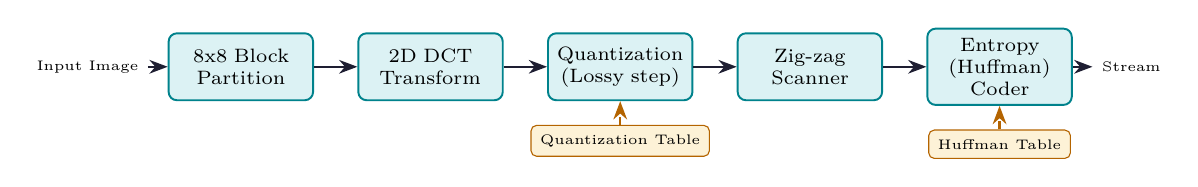
\begin{tikzpicture}[node distance=0.4cm and 0.55cm,
  sblock/.style={rectangle, draw=myteal, fill=hdrteal, text width=1.6cm,
    align=center, minimum height=0.85cm, font=\scriptsize,
    rounded corners=3pt, line width=0.7pt}]
    
  \node (in) at (-0.6, 0) {\tiny Input Image};
  \node[sblock, right=0.25cm of in] (part) {8x8 Block\\Partition};
  \node[sblock, right=of part] (dct) {2D DCT\\Transform};
  \node[sblock, right=of dct] (quant) {Quantization\\(Lossy step)};
  \node[sblock, right=of quant] (zig) {Zig-zag\\Scanner};
  \node[sblock, right=of zig] (ent) {Entropy\\(Huffman) Coder};
  \node (out) [right=0.25cm of ent] {\tiny Stream};
  
  \draw[arrow] (in) -- (part);
  \draw[arrow] (part) -- (dct);
  \draw[arrow] (dct) -- (quant);
  \draw[arrow] (quant) -- (zig);
  \draw[arrow] (zig) -- (ent);
  \draw[arrow] (ent) -- (out);
  
  \node[draw=myamber, fill=hdramber, rectangle, rounded corners=2pt, font=\tiny, below=0.3cm of quant] (qtbl) {Quantization Table};
  \draw[arrow, dashed, color=myamber] (qtbl) -- (quant);
  
  \node[draw=myamber, fill=hdramber, rectangle, rounded corners=2pt, font=\tiny, below=0.3cm of ent] (htbl) {Huffman Table};
  \draw[arrow, dashed, color=myamber] (htbl) -- (ent);
\end{tikzpicture}
\end{tcolorbox}

\begin{enumerate}[leftmargin=*, itemsep=3pt]
  \item \textbf{Image Partitioning:} Divide the image into non-overlapping $8 \times 8$ blocks.
  \item \textbf{DCT:} Apply 2D DCT to each block, producing 1 DC coefficient and 63 AC coefficients.
  \item \textbf{Quantization:} Divide each coefficient by its corresponding entry in a Quantization Table and round to the nearest integer. \textit{This is the only lossy step in JPEG.}
  \item \textbf{Zig-zag Scan:} Re-order the 2D matrix into a 1D vector in a zig-zag path, grouping low-frequency components together and producing long runs of zeros.
  \item \textbf{Entropy Coding:} Compress the values using Run-Length Coding (RLC) and Huffman coding.
\end{enumerate}

\subsection{JPEG-2000 Standard (DWT-Based)}
Instead of DCT, JPEG-2000 uses the \textbf{Discrete Wavelet Transform (DWT)}:
\begin{itemize}[leftmargin=*, itemsep=2.5pt]
  \item Eliminates the "blocking artifacts" visible in JPEG at high compression ratios.
  \item Employs EBCOT (Embedded Block Coding with Optimal Truncation).
  \item Supports progressive transmission (image loads from coarse to fine detail).
\end{itemize}

% ===============================================================================
\section{Worked Examples}
% ===============================================================================

\begin{tcolorbox}[examplebox, title={Huffman Coding Design}]
\textbf{Problem:} A discrete source emits 5 symbols with the following probabilities:
\begin{center}
  \small
  {\renewcommand{\arraystretch}{1.65}%
\begin{tabular}{|c|c|c|c|c|c|}
\hline
Symbol $s_i$ & $s_1$ & $s_2$ & $s_3$ & $s_4$ & $s_5$ \\[4pt]
\hline
Probability $P(s_i)$ & 0.4 & 0.2 & 0.2 & 0.1 & 0.1 \\[4pt]
\hline
\end{tabular}}
\end{center}
\begin{enumerate}[label=(\alph*), leftmargin=*, itemsep=2pt]
  \item Construct the binary Huffman code for each symbol.
  \item Calculate the average code word length $L_{\text{avg}}$.
  \item Compute the source entropy $H(S)$.
  \item Calculate the coding efficiency $\eta$.
\end{enumerate}

\par\noindent\rule{\linewidth}{0.5pt}\par
\textbf{Solution:}

\textbf{(a) Code Word Construction:}
Combine the lowest probabilities recursively:
\begin{itemize}[leftmargin=1.5em, itemsep=2.5pt]
  \item Combine $s_4(0.1)$ and $s_5(0.1) \rightarrow s_{45}(0.2)$.
  \item Sort: $s_1(0.4)$, $s_2(0.2)$, $s_3(0.2)$, $s_{45}(0.2)$.
  \item Combine $s_3(0.2)$ and $s_{45}(0.2) \rightarrow s_{345}(0.4)$.
  \item Sort: $s_1(0.4)$, $s_{345}(0.4)$, $s_2(0.2)$.
  \item Combine $s_{345}(0.4)$ and $s_2(0.2) \rightarrow s_{2345}(0.6)$.
  \item Combine $s_1(0.4)$ and $s_{2345}(0.6) \rightarrow 1.0$.
\end{itemize}
Assigning bits (0 to upper, 1 to lower path):
\begin{itemize}[leftmargin=1.5em, itemsep=2pt]
  \item $s_1 \rightarrow 0$ (length 1)
  \item $s_2 \rightarrow 11$ (length 2)
  \item $s_3 \rightarrow 100$ (length 3)
  \item $s_4 \rightarrow 1010$ (length 4)
  \item $s_5 \rightarrow 1011$ (length 4)
\end{itemize}

\textbf{(b) Average Code Word Length ($L_{\text{avg}}$):}
\begin{equation*}
  L_{\text{avg}} = \sum P(s_i) l_i = 0.4(1) + 0.2(2) + 0.2(3) + 0.1(4) + 0.1(4) = 0.4 + 0.4 + 0.6 + 0.4 + 0.4 = 2.2 \text{ bits/sym}
\end{equation*}

\textbf{(c) Entropy ($H(S)$):}
\begin{align*}
  H(S) &= - \sum P(s_i) \log_2 P(s_i) \\
  &= - [0.4\log_2 0.4 + 2(0.2\log_2 0.2) + 2(0.1\log_2 0.1)] \\
  &= - [0.4(-1.322) + 0.4(-2.322) + 0.2(-3.322)] \\
  &= - [-0.529 - 0.929 - 0.664] = 2.122 \text{ bits/symbol}
\end{align*}

\textbf{(d) Coding Efficiency ($\eta$):}
\begin{equation*}
  \eta = \frac{H(S)}{L_{\text{avg}}} \times 100\% = \frac{2.122}{2.2} \times 100\% \approx 96.45\%
\end{equation*}
\end{tcolorbox}

\newpage

% ===============================================================================
% MANDATORY QUICK REVISION PAGE
% ===============================================================================
\begin{center}
  {\large\bfseries\color{myred} Quick Revision --- Module VI}\\[3pt]
  {\small\color{mydark} Image Compression $|$ PE-EC702B}
\end{center}
\noindent{\color{myred}\rule{\linewidth}{1.2pt}}
\vspace{4pt}

\begin{tcolorbox}[formulabox, title={\textbf{Key Formulas at a Glance}}]
\renewcommand{\arraystretch}{1.3}
\begin{tabularx}{\linewidth}{B{5.0cm} X}Average Code Length & $L_{\text{avg}} = \sum_{i=1}^J P(s_i) l_i$ \\
Source Entropy & $H(S) = - \sum_{i=1}^J P(s_i) \log_2 P(s_i)$ \\
Coding Efficiency & $\eta = \frac{H(S)}{L_{\text{avg}}} \times 100\%$ \\
DPCM Residual Error & $e(n) = f(n) - \hat{f}(n)$ \\
2D Discrete Cosine Trans. & $T(u,v) = \alpha(u)\alpha(v) \sum_{x=0}^{N-1} \sum_{y=0}^{N-1} f(x,y) \cos\left[ \frac{(2x+1)u\pi}{2N} \right] \cos\left[ \frac{(2y+1)v\pi}{2N} \right]$ \\
Compression Ratio & $C_R = \frac{b_{\text{original}}}{b_{\text{compressed}}}$
\end{tabularx}
\tcbset{colbacktitle=myteal, coltitle=white}
\end{tcolorbox}

\begin{tcolorbox}[defbox, title={\textbf{One-Line Definitions}}]
\begin{itemize}[leftmargin=*, itemsep=2.5pt, topsep=0pt]
  \item \textbf{Coding Redundancy:} Redundancy occurring when code word lengths do not match the symbols' probability values.
  \item \textbf{Inter-pixel Redundancy:} Spatial correlation between neighboring pixels where values are highly predictable.
  \item \textbf{Psycho-visual Redundancy:} Visual details that can be eliminated without being noticed by human visual perception.
  \item \textbf{DPCM:} A predictive coding technique that encodes only the difference between actual and predicted pixel values.
  \item \textbf{Lossy Compression:} Compression that yields high ratios by discarding psycho-visual data, preventing exact recovery.
  \item \textbf{Zig-zag Scan:} A scan path in JPEG that orders 2D DCT coefficients to group zero values together for run-length coding.
\end{itemize}
\end{tcolorbox}

\begin{tcolorbox}[exambox, title={\textbf{Frequently Asked / Viva Questions}}]
\begin{enumerate}[leftmargin=*, itemsep=3.5pt, label=\arabic*.]
  \item \Q{What is the difference between lossless and lossy compression?} Lossless compression reconstructs the original image perfectly without any data loss. Lossy compression discards psycho-visual details to achieve much higher compression, but prevents perfect reconstruction.
  \item \Q{Which step in JPEG causes loss of information?} The Quantization step. Dividing the DCT coefficients by the quantization table values and rounding them to integers discards high-frequency details.
  \item \Q{What are blocking artifacts in JPEG?} At high compression ratios, the individual $8 \times 8$ blocks become visible in the reconstructed image as sharp grid discontinuities due to independent block processing.
  \item \Q{Why is DCT preferred over DFT for transform coding?} The DCT has better energy compaction properties and avoids the boundary discontinuities that the DFT introduces, reducing blocking artifacts.
  \item \Q{How does JPEG-2000 eliminate blocking artifacts?} It uses the Discrete Wavelet Transform (DWT) on the entire image (or large tiles) rather than the DCT on small $8 \times 8$ blocks.
  \item \Q{What is prefix code in Huffman coding?} A prefix code is a code in which no code word is a prefix of any other code word, ensuring that the code can be uniquely decoded in real-time.
  \item \Q{Define Shannon's First Source Coding Theorem.} It states that the minimum average code length required to represent a source without distortion is bounded below by the source entropy $H(S)$.
  \item \Q{Explain LZW coding.} It is a dictionary-based, lossless compression method that replaces recurring sequences of symbols with dictionary indices, commonly used in GIF files.
  \item \Q{What is the function of the zig-zag scan in JPEG?} It converts the 2D block of quantized coefficients into a 1D sequence, grouping high-frequency zero coefficients together to optimize Run-Length Encoding.
  \item \Q{How does Arithmetic Coding differ from Huffman Coding?} Huffman coding maps each individual symbol to a bit sequence. Arithmetic coding encodes the entire message as a single fractional value within an interval.
\end{enumerate}
\tcbset{colbacktitle=myteal, coltitle=white}
\end{tcolorbox}

\begin{tcolorbox}[tikzbox, title={JPEG vs. JPEG-2000 Comparison}]
\centering
{\renewcommand{\arraystretch}{1.55}%
\begin{tabularx}{\linewidth}{|>{\bfseries}B{3.2cm}|Y|Y|}
\hline
Attribute & JPEG & JPEG-2000 \\
\hline
Transform Method & Block-based 2D DCT ($8 \times 8$) & Full-image 2D DWT (Wavelet) \\
\hline
Compression artifacts & Blocking artifacts at high compression & Blurring / ringing at high compression \\[4pt]
\hline
Progressive Display & Poor support & High support (resolution scalability) \\
\hline
\end{tabularx}}
\tcbset{colbacktitle=myteal, coltitle=white}
\end{tcolorbox}

\end{document}
